%===============================================================
% main.tex — File chính của báo cáo/đồ án BKU
% Thay các giá trị trong phần CẤU HÌNH bên dưới trước khi dùng.
%===============================================================
\documentclass[12pt, a4paper]{bkureport}
\usepackage{amsmath}

%---------------------------------------------------------------
% CẤU HÌNH — chỉnh tại đây
%---------------------------------------------------------------
\renewcommand{\BKUsubject}{BÁO CÁO ĐỒ ÁN --- EE3037}  % tên môn / loại báo cáo (chỉnh nếu khác)
\newcommand{\TenDeTai}{THIẾT KẾ MÁY ĐO HUYẾT ÁP OSCILLOMETRIC\\ DỰA TRÊN MPX5050 VÀ STM32F103}
\newcommand{\TenGVHD}{(Điền họ tên giảng viên hướng dẫn)}
\newcommand{\TenSVTH}{Phan Trần Thế Huy}
\newcommand{\MSSV}{(Điền MSSV)}
\newcommand{\NgayBaoCao}{tháng 5 năm 2026}
%---------------------------------------------------------------

\begin{document}

	%----- SỐ TRANG LA MÃ (bìa, lời cảm ơn, tóm tắt, mục lục) -----
	\pagenumbering{Roman}

	\include{bia}
	\pagestyle{plain}
	\include{loicamon}
	%===============================================================
% tomtat.tex — Tóm tắt đề tài
%===============================================================
\begin{center}
	\textbf{{\Large\textcolor{black}{TÓM TẮT ĐỀ TÀI}}}
\end{center}

\vspace{1cm}

\hspace*{2cm}
Đề tài trình bày thiết kế một máy đo huyết áp điện tử theo phương pháp \textit{oscillometric}: áp suất trong băng được đo bằng cảm biến áp tuyến tính NXP MPX5050, chuyển đổi tương tự--số qua ADC ngoài Texas Instruments ADS1115 giao tiếp I\textsuperscript{2}C với vi điều khiển STM32F103 (Blue Pill). Firmware điều khiển bơm và van bằng PWM để bơm chậm, ramp đến mục tiêu và xả chậm trong khi đo; đồng thời truyền dòng dữ liệu áp suất khoảng 100 mẫu/giây qua UART (115200~bps) về máy tính.

Phần mềm host (WebApp Vite + TypeScript, Web Serial trên Chrome/Edge) lọc số dải thông 0{,}5--5~Hz, ước lượng áp tâm thu đại diện trong pha bơm chậm để gửi lệnh đặt áp mục tiêu \texttt{T,<mmHg>} xuống MCU; trong pha xả, máy chủ tạo đường bao dao động và áp dụng thuật toán biên độ cực đại (MAA) với các hệ số đặc trưng \(r_s\), \(r_d\) để suy ra MAP, SBP và DBP. Hệ thống có cơ chế an toàn cục bộ: trần áp 280~mmHg, dừng khẩn cấp nút cứng và lệnh \texttt{ABORT}, báo hiệu LED (đỏ/vàng/xanh) theo trạng thái đo.

Kết quả là một nguyên mẫu phần cứng--phần mềm thống nhất phục vụ đo và hiển thị trên trình duyệt; độ chính xác lâm sàng phụ thuộc hiệu chỉnh cảm biến và tinh chỉnh tham số MAA, được nêu trong kết luận và hướng phát triển.


	%----- MỤC LỤC -----
	\pagestyle{empty}
	\tableofcontents
	\clearpage

	%----- DANH MỤC ẢNH -----
	\pagestyle{empty}
	\listoffigures
	\clearpage

	%----- DANH MỤC BẢNG -----
	\pagestyle{empty}
	\listoftables
	\clearpage

	%----- DANH MỤC CHỮ VIẾT TẮT -----
	\chapter*{{\Large\begin{center}DANH MỤC CHỮ VIẾT TẮT\end{center}}}
	%===============================================================
% viettat.tex — Danh mục chữ viết tắt
%===============================================================
\begin{table}[h!]
	\centering
	\begin{tabular}{ll}
		ADC     & Analog-to-Digital Converter (bộ chuyển đổi tương tự--số) \\
		ADS1115 & Bộ ADC Sigma-Delta 16-bit (Texas Instruments) \\
		DBP     & Diastolic Blood Pressure (huyết áp tâm trương) \\
		FSM     & Finite State Machine (máy trạng thái hữu hạn) \\
		HMI     & Human--Machine Interface (giao diện người--máy) \\
		I\textsuperscript{2}C & Giao tiếp nối tiếp hai dây \\
		MAA     & Maximum Amplitude Algorithm (thuật toán biên độ cực đại) \\
		MAP     & Mean Arterial Pressure (huyết áp trung bình động mạch) \\
		MCU     & Microcontroller Unit (vi điều khiển) \\
		MPX5050 & Cảm biến áp tích hợp (NXP) \\
		OWE     & Oscillometric Waveform Envelope (đường bao dao động oscillometric) \\
		PWM     & Pulse Width Modulation (điều chế độ rộng xung) \\
		SAF     & Safety (an toàn -- giới hạn áp cực đại) \\
		SBP     & Systolic Blood Pressure (huyết áp tâm thu) \\
		UART    & Universal Asynchronous Receiver/Transmitter \\
	\end{tabular}
\end{table}

	\pagestyle{empty}
	\clearpage

	%----- CÁC CHƯƠNG NỘI DUNG -----
	\pagenumbering{arabic}
	\pagestyle{fancy}

	% Trang đầu chương cũng có header/footer
	\fancypagestyle{plain}{
		\fancyhf{}
		\fancyhead[L]{\BKUsubject}
		\fancyhead[R]{\leftmark}
		\fancyfoot[C]{\thepage}
		\renewcommand{\headrulewidth}{1pt}
		\renewcommand{\footrulewidth}{1pt}
	}

	%===============================================================
% chap1.tex — Chương 1: Giới thiệu
%===============================================================
\pagestyle{fancy}
\chapter{GIỚI THIỆU}

\section{Tổng quan đề tài}
Đo huyết áp động mạch là một trong các chỉ số sinh lý quan trọng trong chẩn đoán và theo dõi bệnh tim mạch. Trong thực hành lâm sàng cổ điển, phương pháp Korotkoff kết hợp máy đo thủy ngân và ống nghe cho phép xác định áp tâm thu (SBP) và áp tâm trương (DBP) nhờ âm thanh nghe được khi xả khí vòng bít. Máy đo điện tử hiện đại phổ biến thay thế tai nghe bằng việc phân tích dao động áp suất nhỏ trên nền áp suất bao (\textit{oscillometric}), phù hợp với phần cứng chi phí thấp và tái lập trình.

Đề tài xây dựng một nguyên mẫu máy đo oscillometric với các đặc điểm sau:
\begin{itemize}\itemsep0pt \parskip0pt \parsep0pt
	\item \textbf{Cảm biến áp:} MPX5050GP (đầu ra tương tự thuận tiện khuếch đại/đọc ADC).
	\item \textbf{Bộ chuyển đổi số:} ADS1115 độ phân giải 16-bit, giao tiếp I\textsuperscript{2}C với STM32F103.
	\item \textbf{Điều khiển khí nén:} bơm và van được điều chỉnh bằng PWM để đạt tốc độ bơm và xả mong muốn.
	\item \textbf{An toàn:} giới hạn áp suất cực đại 280~mmHg (SAF), dừng khẩn cấp nút cứng và lệnh serial \texttt{ABORT}.
	\item \textbf{Host:} WebApp đọc cổng serial (Web Serial), hiển thị sóng áp và thực hiện lọc số + thuật toán MAA để suy ra MAP, SBP, DBP.
\end{itemize}

\section{Nhiệm vụ đề tài}
\noindent\textbf{Nội dung 1: Phần cứng và bo mạch (OscilloBP Monitor).}\\
\vspace{-0.6cm}
\begin{itemize}\itemsep0pt \parskip0pt \parsep0pt
	\item \textbf{Mục tiêu:} Hoàn thiện mạch đo áp, MCU, điều khiển bơm/van, nút nhấn và LED trạng thái theo schematic/PCB trong kho mã.
	\item \textbf{Ý tưởng thực hiện:} MPX5050 cấp điện áp tỉ lệ áp suất; ADS1115 lấy mẫu ổn định hơn ADC nội Blue Pill; STM32 điều phối FSM đo và streaming UART.
\end{itemize}
\vspace{-0.2cm}

\noindent\textbf{Nội dung 2: Firmware STM32 (PlatformIO / STM32Cube).}\\
\vspace{-0.6cm}
\begin{itemize}\itemsep0pt \parskip0pt \parsep0pt
	\item \textbf{Mục tiêu:} Đọc áp liên tục trong các pha đo, điều khiển bơm/van theo tốc độ đặt trước, đồng bộ với lệnh \texttt{T,...} từ host.
	\item \textbf{Ý tưởng thực hiện:} Máy trạng thái gồm các pha bơm chậm (nghe dao động), ramp margin, xả chậm đo, xả nhanh kết thúc hoặc an toàn; định dạng khung \texttt{S,<seq>,<t\_ms>,<p\_mmHg>} và thông báo \texttt{A,...}, \texttt{E,...}.
\end{itemize}
\vspace{-0.2cm}

\noindent\textbf{Nội dung 3: Phần mềm host và kiểm chứng.}\\
\vspace{-0.6cm}
\begin{itemize}\itemsep0pt \parskip0pt \parsep0pt
	\item \textbf{Mục tiêu:} Hiển thị thời gian thực, lọc dao động, tính MAP/SBP/DBP bằng MAA; kiểm thử UART, LED và SAF.
	\item \textbf{Ý tưởng thực hiện:} Band-pass 0{,}5--5~Hz trên chuỗi áp; phát hiện dao động đầu tiên trong pha bơm chậm để ước lượng \texttt{P\_sys\_est} và gửi \texttt{T,P\_sys\_est+margin}.
\end{itemize}

\section{Bố cục báo cáo}
Ngoài phần đầu (tóm tắt, mục lục, danh mục hình/bảng và viết tắt), báo cáo gồm bốn chương chính và phần kết luận. \textbf{Chương 2} trình bày kiến trúc phần cứng và hình ảnh schematic/in PCB. \textbf{Chương 3} mô tả firmware, giao thức serial và cơ sở thuật toán oscillometric/MAA được triển khai trên host. \textbf{Chương 4} giới thiệu WebApp và checklist kiểm thử. \textbf{Kết luận} tóm tắt kết quả, hạn chế và hướng phát triển.

	%===============================================================
% chap2.tex — Phần cứng
%===============================================================
\pagestyle{fancy}
\chapter{CƠ SỞ PHẦN CỨNG}

\section{Sơ đồ khối chức năng}
Hệ thống gồm các khối sau:
\begin{enumerate}\itemsep0pt
	\item \textbf{Vòng bít và đường khí nối:} chứa áp suất làm xẹp động mạch và truyền áp tới cảm biến.
	\item \textbf{Cảm biến MPX5050:} chuyển áp suất tương đối thành điện áp tương tự (khảo sát đường đặc tuyến trong datasheet).
	\item \textbf{ADC ADS1115:} chuyển đổi điện áp với độ phân giải 16-bit; giao tiếp I\textsuperscript{2}C với MCU (địa chỉ thiết bị mặc định 0x48 khi chân ADDR nối GND).
	\item \textbf{Vi điều khiển STM32F103 (Blue Pill):} đọc ADS1115, điều khiển PWM bơm và van, đọc nút nhấn, điều khiển LED và truyền thông UART.
	\item \textbf{Nguồn và điều kiện tiếp đất:} đảm bảo MPX5050 và ADC có tham chiếu ổn định; layout PCB tuân thủ khuyến nghị của nhà sản xuất để giảm nhiễu đo lường.
\end{enumerate}

\section{Giao tiếp và chân cắm chính}
Theo cấu hình mặc định trong firmware (\texttt{board\_config.h}):
\begin{itemize}\itemsep0pt
	\item UART1 115200~bps: PA9 (TX), PA10 (RX).
	\item I2C1: PB6 (SCL), PB7 (SDA) nối ADS1115.
	\item Timer 3 PWM: PA6 kênh bơm, PA7 kênh van (điều chỉnh duty để servo tốc độ bơm/xả).
	\item Nút tác động mức thấp (kéo lên nội bộ): PA3 Start, PA4 Stop, PA5 High-mode.
	\item LED báo hiệu: PB13 đỏ, PB14 xanh, PB15 vàng (ánh xạ trạng thái đo và cảnh báo).
\end{itemize}

\section{An toàn và giới hạn vật lý}
\begin{itemize}\itemsep0pt
	\item Trần áp \textbf{280~mmHg}: firmware ngắt bơm và mở van để xả nhanh khi vượt ngưỡng hoặc khi người dùng nhấn Stop/\texttt{ABORT}.
	\item Timeout rò khí: nếu áp không tăng đủ trong khoảng thời gian đặt (ví dụ rò đường khí), FSM báo lỗi cảm biến/rò và chuyển LED đỏ báo lỗi.
\end{itemize}

\section{Schematic và PCB}
Thiết kế schematic và bản vẽ PCB được hoàn thiện trong dự án KiCad \textit{OscilloBP Monitor}. Hình~\ref{fig:schematic-print} trích bản in PDF trong kho mã (có thể thay bằng ảnh độ phân giải cao hơn khi cần in báo cáo).

\begin{figure}[htbp]
	\centering
	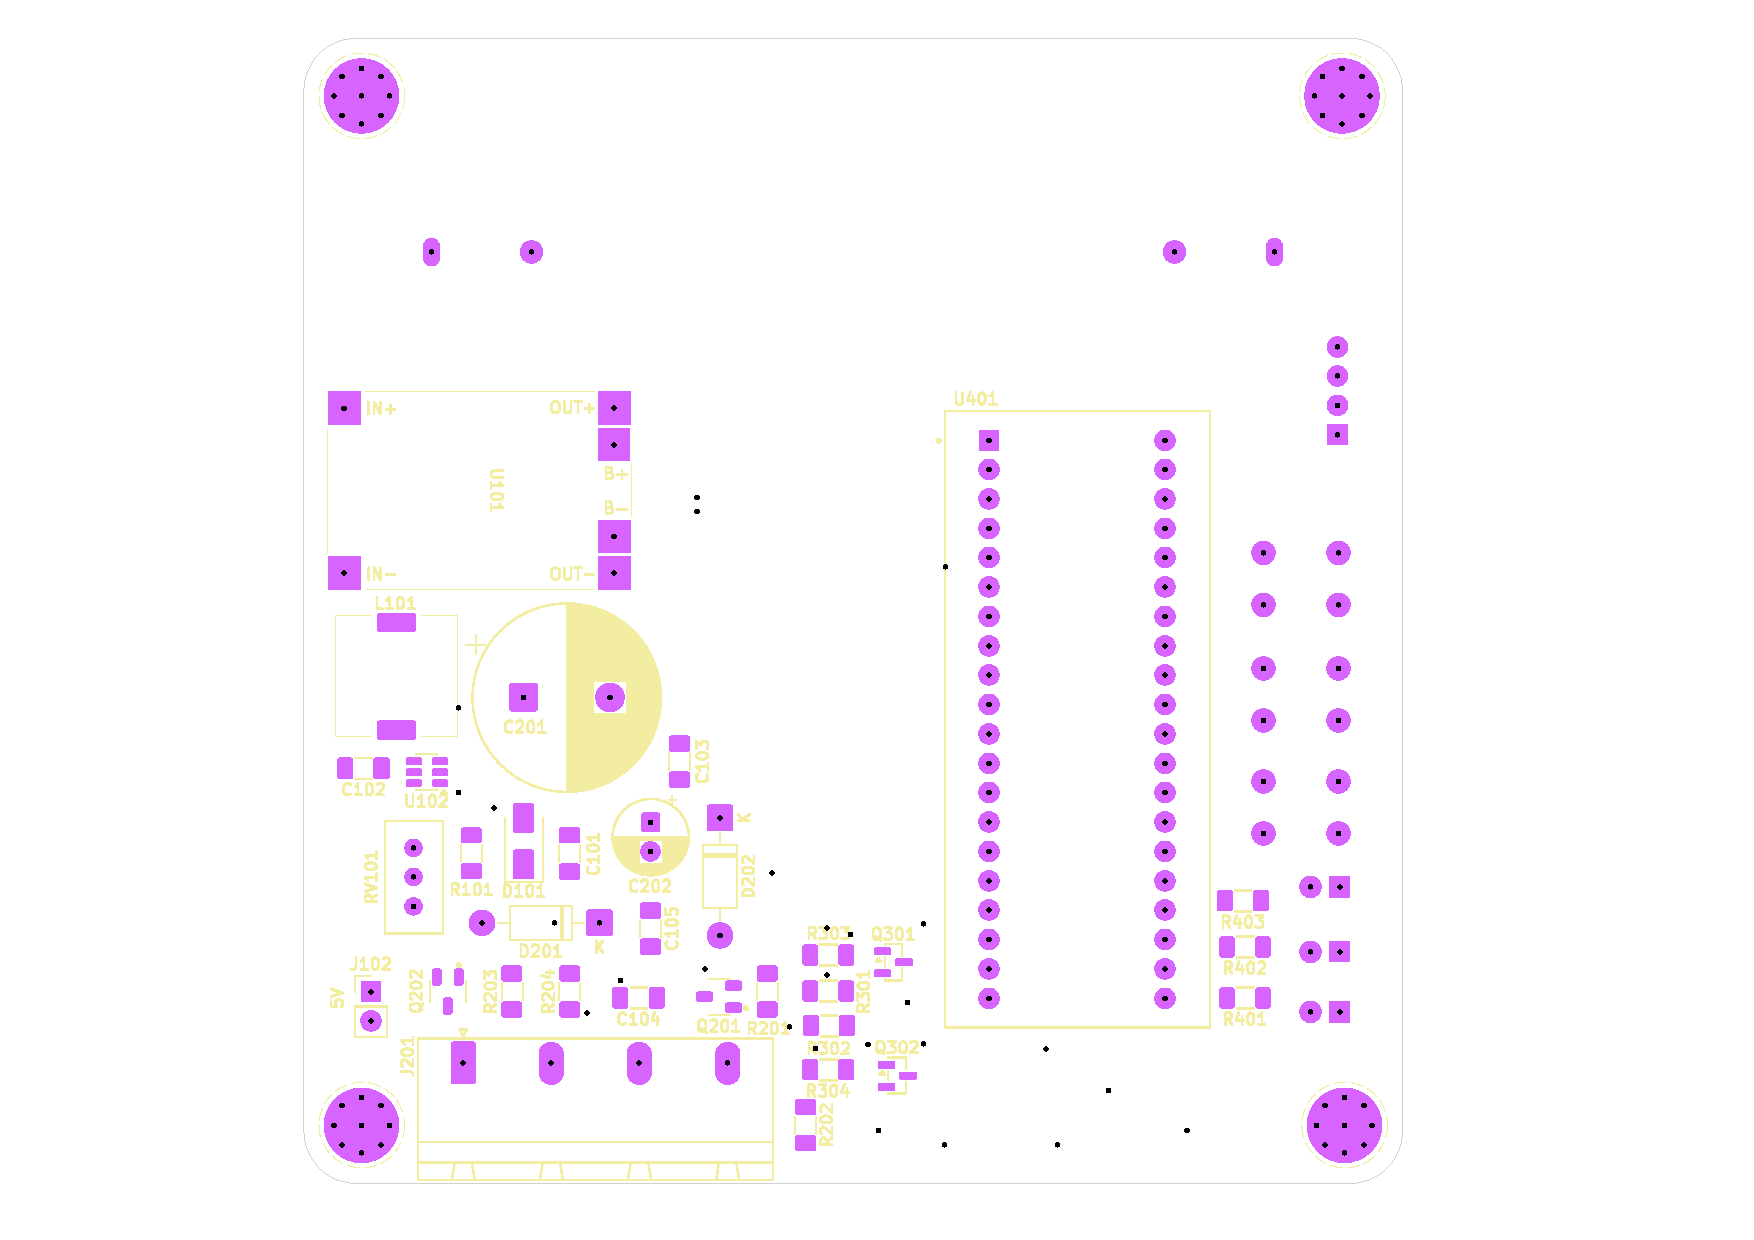
\includegraphics[width=0.95\textwidth]{images/schematic-print.pdf}
	\caption{Bản in schematic/board (trích từ dự án KiCad OscilloBP Monitor).}
	\label{fig:schematic-print}
\end{figure}

\section{Nhiệm vụ hiệu chỉnh phần cứng}
Để đọc mmHg chính xác từ ADC, cần hiệu chỉnh hai tham số trong firmware: \texttt{PRESSURE\_ADC\_OFFSET\_COUNTS} và \texttt{PRESSURE\_ADC\_SCALE\_MMHG\_PER\_COUNT} so với đồng hồ áp chuẩn hoặc nguồn áp đã biết. Đây là bước bắt buộc trước khi đánh giá lâm sàng.

	%===============================================================
% chap3.tex — Firmware và thuật toán
%===============================================================
\pagestyle{fancy}
\chapter{FIRMWARE VÀ THUẬT TOÁN OSCILLOMETRIC}

\section{Kiến trúc phần mềm nhúng}
Firmware được xây dựng bằng PlatformIO, board \texttt{bluepill\_f103c8}, framework STM32Cube HAL. Các module chính:
\begin{itemize}\itemsep0pt
	\item Driver ADS1115 đọc kênh vi sai phù hợp với điện áp ra của MPX5050 và PGA đặt trong phạm vi đầy thang không bão hòa.
	\item Chuyển đổi đếm ADC \(\rightarrow\) áp suất cuff (mmHg) bằng offset và hệ số scale (hiệu chỉnh thực nghiệm).
	\item FSM đo huyết áp: pha bơm chậm có ``nghe'' dao động; pha ramp đến mục tiêu sau lệnh host; pha xả chậm để thu sóng oscillometric; pha xả nhanh kết thúc hoặc an toàn.
	\item UART text-line: stream mẫu và thông báo trạng thái cho WebApp.
\end{itemize}

\section{Luồng đo và giao thức UART}
Bảng~\ref{tab:uart-frames} tóm tắt các khung điển hình (chi tiết trong tài liệu \texttt{pc-bridge.md} của kho mã).

\begin{table}[htbp]
	\centering
	\caption{Các dòng lệnh/thông báo UART tiêu biểu.}
	\label{tab:uart-frames}
	\begin{tabular}{ll}
		\hline
		\textbf{Dòng} & \textbf{Ý nghĩa} \\
		\hline
		\texttt{S,<seq>,<t\_ms>,<p\_mmHg>} & Stream áp suất (~100 Hz trong đo) \\
		\texttt{A,IDLE} / \texttt{A,INFLATE\_SLOW} / \texttt{A,DEFLATE} & Trạng thái FSM \\
		\texttt{T,<target\_mmHg>} & Host đặt áp mục tiêu (clamp \(\leq\) SAF) \\
		\texttt{ABORT} hoặc \texttt{A} & Yêu cầu xả nhanh an toàn \\
		\texttt{E,MEAS\_END} & Kết thúc đo \\
		\hline
	\end{tabular}
\end{table}

Tốc độ nền: baud 115200, kết thúc dòng \texttt{\textbackslash r\textbackslash n}. Trần SAF \textbf{280~mmHg} áp dụng đồng nhất cho điều khiển cục bộ và clamp lệnh \texttt{T,...}.

\section{Cơ sở thuật toán MAA trên host}
Thuật toán biên độ cực đại (MAA) làm việc trên đường bao dao động (OWE) của thành phần AC của áp suất cuff trong quá trình xả chậm:
\begin{enumerate}\itemsep0pt
	\item Xác định \(\mathrm{MAP}\) là áp suất cuff tại điểm biên độ dao động cực đại \(A_{\max}\).
	\item Với các hệ số đặc trưng \(r_s\) (tâm thu) và \(r_d\) (tâm trương), tính các mức biên độ mục tiêu \(A_{\mathrm{sys}} = r_s A_{\max}\), \(A_{\mathrm{dia}} = r_d A_{\max}\).
	\item Dò nhánh áp cao hơn MAP để tìm điểm gần \(A_{\mathrm{sys}}\) \(\Rightarrow\) SBP; dò nhánh áp thấp hơn MAP để tìm điểm gần \(A_{\mathrm{dia}}\) \(\Rightarrow\) DBP.
\end{enumerate}

Trên host, trước khi trích envelope và cực đại, tài liệu kỹ thuật dự án khuyến nghị \textbf{lọc số dải thông 0{,}5--5~Hz} để giữ nhịp mạch và giảm nhiễu tay/run.

\section{Đồng bộ với pha bơm chậm}
Trong pha \texttt{INFLATE\_SLOW}, WebApp theo dõi dao động sau lọc để ước lượng \(\mathrm{P\_sys\_est}\). Sau đó host gửi \(\texttt{T},\mathrm{P\_sys\_est}+40\) (margin mặc định trong \texttt{board\_config.h}) để MCU ramp đến mục tiêu rồi chuyển xả chậm đo. Nếu không có host trong thời gian chờ, firmware có thể ramp theo mục tiêu dự phòng (\texttt{INFLATE\_FALLBACK\_TARGET\_MMHG}).

\section{LED và trải nghiệm người dùng}
LED phản ánh trạng thái không chặn luồng đo (tham chiếu \texttt{LED\_Algorithm.md}): idle/done xanh; bơm margin vàng nhấp nháy; đo/xả vàng sáng; STOP/SAF/\texttt{ABORT} đỏ nhấp nháy nhanh; lỗi rò/I2C đỏ sáng.

	%===============================================================
% chap4.tex — Phần mềm host và kiểm thử
%===============================================================
\pagestyle{fancy}
\chapter{PHẦN MỀM HOST VÀ KIỂM THỬ}

\section{WebApp và Web Serial}
Ứng dụng web (\texttt{Software/webapp}) dùng Vite và TypeScript, chạy trên trình duyệt Chrome hoặc Edge với API Web Serial để mở cổng USB--TTL nối UART của MCU. Giao diện hiển thị sóng áp thời gian thực và các nút điều khiển (\textbf{Hủy} gửi \texttt{ABORT}; ô kiểm SAF có thể minh họa clamp khi gửi \texttt{T,300}).

\begin{figure}[htbp]
	\centering
	
\includegraphics[width=0.92\textwidth]{images/webapp-hero.png}
	\caption{Minh họa giao diện WebApp (ảnh hero trong kho mã).}
	\label{fig:webapp}
\end{figure}

\section{Xử lý tín hiệu trên host}
Luồng xử lý khuyến nghị:
\begin{enumerate}\itemsep0pt
	\item Thu thập chuỗi mẫu áp từ các dòng \texttt{S,...}.
	\item Áp dụng lọc dải thông 0{,}5--5~Hz để cô lập dao động pulsatile.
	\item Trong bơm chậm: phát hiện dao động đạt ngưỡng đủ lớn để ghi \(\mathrm{P\_sys\_est}\).
	\item Gửi \(\texttt{T},\mathrm{P\_sys\_est}+\mathrm{margin}\) xuống MCU.
	\item Trong xả chậm: xây envelope và chạy MAA để hiển thị MAP/SBP/DBP.
\end{enumerate}

\section{Kiểm thử được khuyến nghị}
Checklist trong \texttt{Firmware/TESTING.md} và \texttt{Firmware/testcase.md} hướng dẫn các nhóm thử:

\noindent\textbf{Nhóm an toàn (SAF):}
\begin{itemize}\itemsep0pt
	\item STOP khi đang bơm: bơm tắt ngay, van mở tối đa, LED đỏ nhấp nháy nhanh.
	\item Trần 280~mmHg: MCU cắt bơm và báo động.
	\item Lệnh \texttt{T,300}: firmware clamp về 280.
	\item \texttt{ABORT}/\texttt{A}: xả nhanh như STOP phần cứng về hành vi an toàn.
\end{itemize}

\noindent\textbf{Nhóm UART:}
\begin{itemize}\itemsep0pt
	\item Kiểm tra ~100 khung \texttt{S,...}/giây trong inflate/deflate.
	\item Sau \texttt{T,...}, MCU vào margin rồi xả đo đúng trình tự.
\end{itemize}

\noindent\textbf{Nhóm LED/HMI:} idle xanh; inflate vàng nhấp nháy \(\sim\)500~ms; đo/xả vàng sáng; STOP/SAF/fast deflate đỏ nhấp nháy \(\sim\)150~ms; lỗi rò/I2C đỏ sáng.

\section{Hạn chế của kiểm thử trong phòng lab}
 Firefox/Safari không hỗ trợ Web Serial; có thể cần bridge TCP/\texttt{socat} nếu phải dùng trình duyệt khác. Đánh giá độ chính xác lâm sàng đòi hiệu chỉnh đồng hồ áp và mẫu đối chứng đủ lớn, nằm ngoài phạm vi một checklist chức năng thuần túy.


	%----- KẾT LUẬN & TÀI LIỆU THAM KHẢO -----
	\fancypagestyle{plain}{
		\fancyhf{}
		\fancyfoot[C]{\thepage}
		\renewcommand{\headrulewidth}{0pt}
		\renewcommand{\footrulewidth}{0pt}
	}
	\pagestyle{plain}
	%===============================================================
% ketluan.tex — Kết luận
%===============================================================
\chapter*{{\Large\begin{center}KẾT LUẬN\end{center}}}
\addcontentsline{toc}{chapter}{Kết luận}

\section*{Kết quả đạt được}
Đề tài đã xây dựng được một nguyên mẫu máy đo huyết áp oscillometric với đầy đủ các khối chức năng: cảm biến MPX5050, ADC ADS1115, vi điều khiển STM32F103 điều khiển bơm/van PWM và streaming UART; phần mềm WebApp trên trình duyệt hỗ trợ Web Serial để hiển thị sóng áp, lọc số và MAA nhằm suy ra MAP, SBP và DBP; cơ chế an toàn trần áp 280~mmHg và dừng khẩn cấp được triển khai đồng thời trên firmware và qua lệnh serial. Bo mạch và schematic được thể hiện trong dự án KiCad OscilloBP Monitor kèm Gerber phục vụ gia công.

\section*{Hạn chế}
Độ chính xác tuyệt đối phụ thuộc mạnh vào hiệu chỉnh offset/scale của kênh đo áp và vào bộ hệ số \(r_s\), \(r_d\) của MAA; các giá trị mặc định trong tài liệu chỉ mang tính tham chiếu và cần tinh chỉnh theo dữ liệu lâm sàng hoặc bộ phép đo chuẩn. Web Serial giới hạn loại trình duyệt; đo trong điều kiện chuyển động tay hoặc nhiễu điện từ có thể làm méo envelope nếu không bổ sung lọc/outlier mạnh hơn.

\section*{Hướng phát triển}
Áp dụng hiệu chỉnh đa điểm và lưu hệ số trên EEPROM; mở rộng thuật toán (khớp đường cong Gauss, thích ứng \(r_s,r_d\)); tích hợp bridge TCP/WebSocket cho đa nền tảng; thực hiện thử nghiệm so sánh với máy đo đã chứng nhận y tế và hoàn thiện hồ sơ an toàn điện/khí nén cho sản phẩm.

	\captionsetup{labelformat=empty}
	% LTeX: enabled=false
%===============================================================
% tlthamkhao.tex — Tài liệu tham khảo
%===============================================================
\begin{thebibliography}{99}

	\bibitem{mpx5050}
	NXP Semiconductors,
	\textit{MPX5050 / MPX5050GP --- Integrated Silicon Pressure Sensor On-Chip Signal Conditioned, Temperature Compensated and Calibrated},
	Datasheet, truy cập qua trang nhà sản xuất.

	\bibitem{ads1115}
	Texas Instruments,
	\textit{ADS1113, ADS1114, ADS1115 --- Ultra-Small, Low-Power, I\textsuperscript{2}C-Compatible, 860-SPS ADC With Internal Reference},
	Datasheet SBAS444.

	\bibitem{stm32f103}
	STMicroelectronics,
	\textit{STM32F103x8 / STM32F103xB --- Medium-density performance line ARM-based 32-bit MCU},
	Reference Manual RM0008 và Datasheet DS5319.

	\bibitem{geddes}
	L.\ A.\ Geddes và M.\ Voelz,
	\textit{Pulse Transit Time as an Indicator of Arterial Blood Pressure},
	và các tài liệu cổ điển về oscillometry / characteristic ratios (tham khảo trong giáo trình đo lường y sinh).

	\bibitem{repo}
	Nhóm dự án,
	\textit{mpx5050-blood-pressure-monitor} --- firmware PlatformIO, WebApp và tài liệu nội bộ (\texttt{algorithm.md}, \texttt{pc-bridge.md}, \texttt{TESTING.md}),
	Kho mã nguồn GitHub \texttt{phantranthehuy/mpx5050-blood-pressure-monitor}, 2026.

\end{thebibliography}


\end{document}
